%\documentclass[11pt,a4paper]{report}
\documentclass[11pt,a4paper]{article}
%\documentclass[11pt,a4paper]{amsart}

% 1 inch margins
\usepackage{fullpage}
\usepackage{framed}
\usepackage{listings}
  \usepackage{courier}
\usepackage{amsmath}
\usepackage{verbatim}
\usepackage{graphicx}
\usepackage[dvips,usenames,dvipsnames]{color}
\usepackage[dvipdf]{hyperref}

\definecolor{codeblock}{rgb}{0.95,0.98,1.0}
%\definecolor{keywords}{rgb}{1.0,0.3,0.0}
\definecolor{keywords}{rgb}{1.0,0.1,1.0}
%\definecolor{comments}{rgb}{0.0,0.7,0.8}
\definecolor{comments}{rgb}{1.0,0.0,0.0}
\definecolor{identifiers}{rgb}{0.1,0.0,1.0}
\definecolor{strings}{rgb}{0.0,0.6,0.0}
\definecolor{basic}{rgb}{0.0,0.4,0.0}

\definecolor{shadecolor}{rgb}{0.9,0.9,0.1}

\lstset{
language=,
%xleftmargin=2em,
%frame=single,
backgroundcolor=\color{codeblock},
basicstyle=\color{basic}\footnotesize\ttfamily,
identifierstyle=\color{identifiers},
keywordstyle=\color{keywords},
commentstyle=\color{comments},
stringstyle=\color{strings},
showstringspaces=false,
%numbers=left,
%numberstyle=\color{Gray}
}

\lstdefinelanguage{cylctaskdef}
{
morekeywords={NAME,DESCRIPTION,TYPE,CONTACT_DELAY,OWNER,CYCLES,TASK,ENVIRONMENT,ESTIMATED_RUN_TIME,PREREQUISITES,STARTUP_PREREQUISITES,OUTPUTS,ESTIMATED_RESTART_OUTPUT_TIMES,NO_NONCOTEMPORAL_DEPENDANTS,ONEOFF_FOLLOW_ON},
sensitive=false,
morecomment=[l]{\#},
morestring=[b]\",
}

\lstdefinelanguage{usage}
{
morekeywords={},
string=[b]{"},
sensitive=false,
morecomment=[l]{Usage:},
morecomment=[l]{Arguments:},
morecomment=[l]{Options:},
morecomment=[l]{Commands:},
morecomment=[l]{usage:},
morecomment=[l]{arguments:},
morecomment=[l]{command-options:},
morecomment=[l]{COMMANDS:},
morecomment=[l]{options:},
}


%\title{Cylc: A Self-Organising Forecast Systems Scheduler with Optimal
%Multi-cycle Catchup Capability [DRAFT:cylc-0.9.0.1]}

\title{Cylc: A Self-Organising Optimal Multicycle Scheduler for Forecast Systems \linebreak Version -CYLC-VERSION-}

\author{Hilary Oliver, NIWA}

\begin{document}

\maketitle

\pagebreak
\tableofcontents
\pagebreak

\begin{abstract}

    {\em Cylc} (pronounced ``silk'') is a self-organising
    metascheduler\footnote{A metascheduler determines when dependent
    jobs are {\em ready} to run, at which point they can be sent to a
    batch queue scheduler. We drop the ``meta'' prefix from here on,
    however, because a metascheduler is also a type of scheduler. The
    term is also used to refer to a single aggregate view of multiple
    distributed resource managers, but that is not the topic of this
    document.} for cycling environmental forecast systems that may include
    many linked scientific models and associated data processing
    tasks.\footnote{A {\em task} is any group of processes treated as a
    single entity for scheduling purposes.} Its novel scheduling
    algorithm maintains an evolving pool of task proxy objects that
    interact with each other to resolve all dependencies so that correct
    scheduling emerges naturally at run time.  Each task is defined in
    isolation and knows just its own prerequisites (but not who will
    satisfy them) and outputs (but not who will use them), and there is
    no need for a global ``suite'' that specifies dependencies or
    execution order. Because cylc does not use global time loops to
    advance the system and treats all dependencies equally, including
    those between tasks in different forecast cycles,\footnote{For our
    purposes a {\em forecast cycle} comprises all tasks with a common
    {\em cycle time}, i.e.\ the analysis time or nominal start time of a
    forecast model, or that of the forecast model(s) associated with the
    other tasks.} it can run tasks from multiple forecast cycles at once
    to the full extent allowed by intercycle dependencies. This matters
    in particular whenever the external driving data\footnote{Forecast
    systems are typically driven by observational data and/or timely
    model fields from an external forecasting system.} for upcoming
    cycles are available in advance: cylc systems can catch up from
    delays very quickly, parallel test systems can be started or
    restarted behind the main operation to catch up as quickly as
    possible, and historical case studies can achieve sustained maximal
    throughput. Delayed and real time operation merge seamlessly in
    cylc: if a system happens to be running behind it will automatically
    achieve optimal multi-cycle scheduling, and when (or if) it catches
    up to real time operation a series of distinct forecast cycles will
    naturally emerge. Cylc is easily interfaced to existing tasks and is
    extremely flexible and easy to use. It can be stopped and restarted
    in arbitrarily complex states of operation and dynamically adapts to
    insertion or removal of tasks. If a task fails and delays its
    downstream dependants the rest of the system will carry on
    unaffected while the problem is addressed, after which time the
    delayed tasks will catch up as quickly as possible.  Cylc's handling
    of forecast model ``restart'' dependencies allows continued
    operation, with very little operator intervention, over major
    failures that result in omitted forecasts in the driving models.
    Ability to control the configured task set, and failure recovery
    scenarios, can be completely tested in an accelerated simulation
    mode that is indistinguishable (to cylc) from real operation. Cylc
    is written in object oriented Python and uses {\em
    Pyro}\footnote{Pyro (Python Remote Objects) is an objected oriented
    Remote Procedure Call technology, copyright Irmen de Jong,
    distributed under the MIT open source license (see
    Section~\ref{Pyro}).} to control tasks across heterogenous
    distributed networks.  

    %\footnote{Cylc also
    %enables new modes of real time operation, for example a catchment
    %river model that runs hourly assimilating real time stream flow
    %observations and using the {\em most recent} 6-hourly precipitation
    %forecast - see EcoConnect, below).} 
\end{abstract}

\pagebreak
\section{How Cylc Works} 
\label{HowCylcWorks}

\subsection{Scheduling For Forecast Systems} 
\label{SchedulingForForecastSystems}

Environmental forecasting systems generate forecast products at regular
intervals using potentially large sets of scientific models and
associated data processing tasks. They are constrained by availability
of external driving data, typically real time observations and/or model
data from an external forecasting system, which one or more tasks depend
on, and these drive other ``downstream'' tasks, and so on. The
dependency diagram for such a system consists of one or more (possibly
linked) {\em Directed Acyclic Graphs}, which may vary according to the
{\em forecast cycle} (wherein each task has the same {\em cycle time},
namely the nominal analysis time or start time of the forecast models in
the group). Normal real time operation necessarily consists of a series
of distinct forecast cycles that are each initiated, after a gap in
processing, by arrival of new external driving data.

From a job scheduling perspective task execution order must be carefully
controlled in order to avoid dependency violations. Ideally, each task
should be queued for execution at the instant its last prerequisite is
satisfied; this is the best that can be done even if queued tasks are
not able to execute immediately because of resource contention.


\subsection{An Example: EcoConnect} 
\label{AnExampleEcoConnect}

This work was motivated by the EcoConnect Forecasting System at NIWA
(National Institute of Water and Atmospheric Research, New Zealand). As
of 2009, EcoConnect takes real time atmospheric and stream flow
observations, and operational global weather forecasts from the Met
Office (UK), and uses these to drive global sea state and regional data
assimilating weather models, which in turn drive regional sea state,
storm surge, and catchment river models, plus tide prediction, and a
large number of associated data collection, quality control,
preprocessing, postprocessing, product generation, and archiving
tasks.\footnote{Future plans for EcoConnect include additional
deterministic regional weather forecasts and a statistical ensemble.}
The global sea state forecast runs once daily.  The regional weather
forecast runs four times daily but it supplies surface pressures to
several downstream models that run only twice daily, and precipitation
accumulations to catchment river models that run on an hourly cycle
assimilating real time stream flow observations and using the most
recent available regional weather forecast.  EcoConnect runs on
heterogenous distributed hardware, including a massively parallel
supercomputer and several Linux servers. 

\subsection{Intracycle Dependencies} 
\label{IntracycleDependencies}

We normally think of dependencies as occuring between tasks within a
forecast cycle. A sea state forecast, for example, might depend on
surface wind fields generated by a weather forecast over the same
forecast range, and a postprocessing task clearly cannot run before its
input data has been generated. Figure~\ref{fig-dep-one} shows the
dependency diagram for a single forecast cycle of a simple example
system consisting of three forecast models ({\em a, b,} and {\em c}) and
three post processing or product generation tasks ({\em d, e} and {\em
f}).  A scheduler capable of handling this must manage, within a single
forecast cycle, multiple parallel streams of execution that branch when
one task generates output for several downstream tasks, and merge when
one task takes input from several upstream tasks. 

\begin{figure} \label{fig-dep-one} 
    \begin{center}
        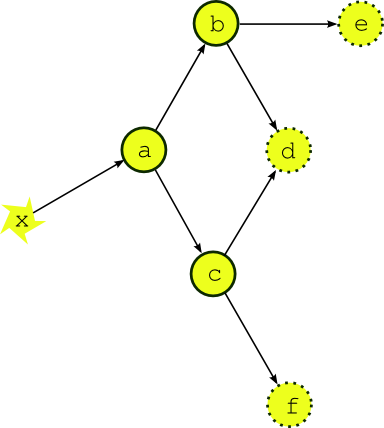
\includegraphics[width=6cm]{inkscape-svg/dep-one-cycle} 
    \end{center}
    \caption{\small Dependency graph for a single forecast cycle of a
    simple example system. Tasks {\em a, b,} and {\em c} represent
    forecast models, {\em d, e} and {\em f} are post processing or
    product generation tasks, and {\em x} represents {\em external
    driving data} that the upstream forecast model depends on.}
\end{figure} 

\begin{figure} \label{fig-time-one}
    \begin{center}
        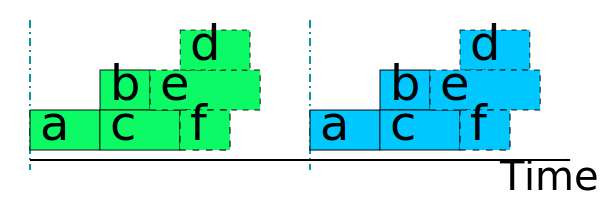
\includegraphics[width=8cm]{inkscape-svg/timeline-one}
    \end{center}
    \caption{\small Job schedule for two consecutive cycles of
the example system during real time operation. The horizontal extent of
each task bar represents its execution time, and the vertical blue lines
show when the external driving data becomes available.}
\end{figure}

Figure~\ref{fig-time-one} shows the job schedule for two consecutive
cycles of the example system in real time operation, given execution
times represented by the horizontal extent of the task bars. There is a
time gap between cycles as the system waits on new external driving
data.  Each task in the example system happens to trigger off upstream
tasks {\em finishing}, rather than some intermediate output or event,
but this is merely a simplification that makes for clearer diagrams.

\begin{figure} \label{fig-dep-two-linked}
    \begin{center}
        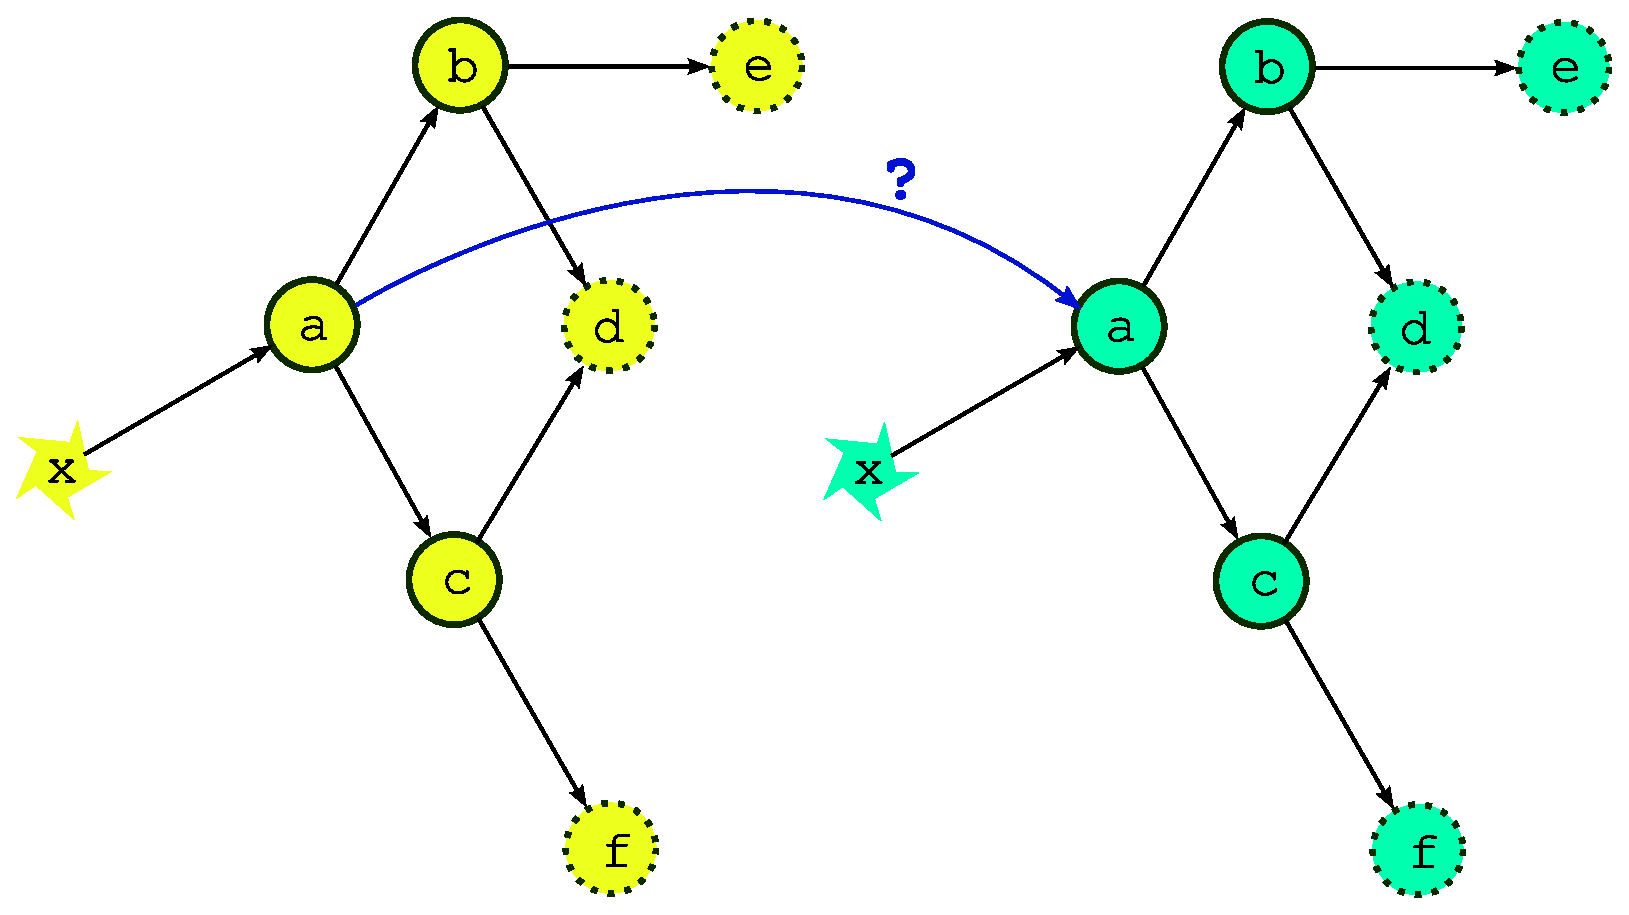
\includegraphics[width=10cm]{inkscape-svg/dep-two-cycles-linked} 
    \end{center}
    \caption{\small If the external driving data is available in
    advance, can we start running the next cycle early?} 
\end{figure}

\subsection{Intercycle Dependencies} 
\label{IntercycleDependencies}

There are also dependencies between tasks in different cycles: forecast
models typically depend on their own most recent previous forecast for
an initial ``background state'', and different types of tasks in
different forecast cycles can also be linked (e.g.\ the complicated
relationship between the catchment river and weather models in
EcoConnect). In real time operation these intercycle dependencies can be
ignored because they are automatically satisfied when each cycle
necessarily finishes before the next one begins. This is just as well
because they dramatically increase the complexity of the dependency
graph of even the simplest systems, by destroying the clean boundary
between forecast cycles. Figure~\ref{fig-dep-two} illustrates the
problem for our simple example system assuming the least intercycle
dependence likely to be present: the forecast models ($a$, $b$, and $c$)
each depend on their own previous instances.

As far as the author is aware existing schedulers ignore intercycle
dependencies and therefore require a series of distinct forecast cycles
at all times. While this fits with our intuitive view of forecasting
systems, based on normal real time operations, it is a serious
impediment when advance availability of external driving data makes it
possible, in principle, to run some tasks from upcoming cycles before
the current cycle is finished. This occurs after delays (late arrival of
external data, system maintenance, etc.) and, to an even greater extent,
in historical case studies, and parallel test systems that are delayed
with respect to the main operation. It is in fact a serious problem for
systems that have little downtime between forecast cycles and
consequently take many cycles to catch up after a delay. If intercycle
dependencies are ignored the best that can be done, in general, is to
reduce the gap between cycles to zero. A limited crude overlap of the
single cycle job schedule may be possible for specific task sets in
certain circumstances, but this is very much sub-optimal and it would be
difficult to guarantee that dependencies will never be violated.

\begin{figure} \label{fig-overlap}
    \begin{center}
        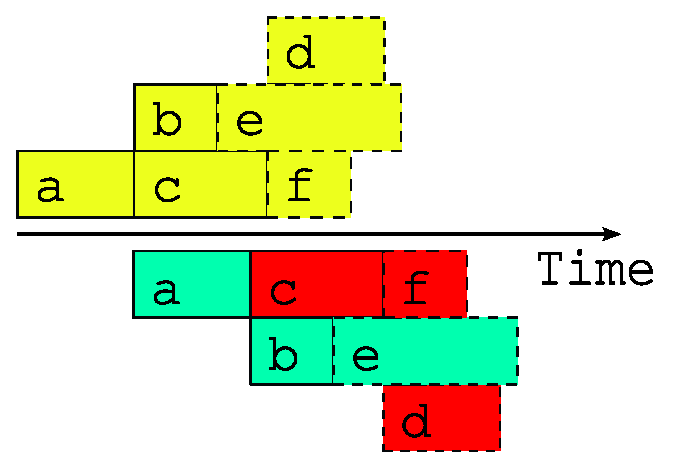
\includegraphics[width=6cm]{inkscape-svg/timeline-one-c} 
    \end{center}
    \caption{\small A naive attempt to overlap two consecutive cycles
    using the single-cycle dependency graph. The red shaded tasks will
    fail because of dependency violations (or will not be able to run
    because of upstream dependency violations).} 
\end{figure} 

\begin{figure} \label{fig-foo}
    \begin{center}
        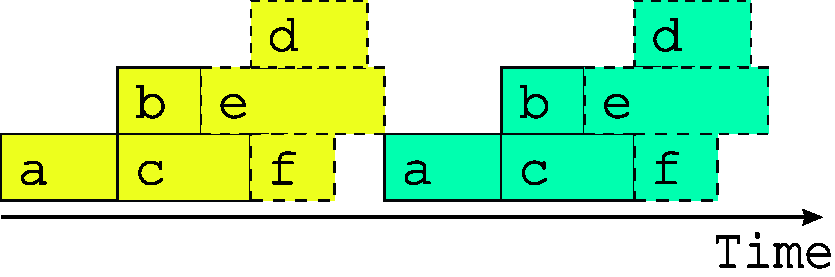
\includegraphics[width=8cm]{inkscape-svg/timeline-one-a} 
    \end{center}
    \caption{\small The best that can be done in general when intercycle dependencies 
    are ignored.} 
\end{figure} 

\begin{figure} \label{fig-dep-two}
    \begin{center}
        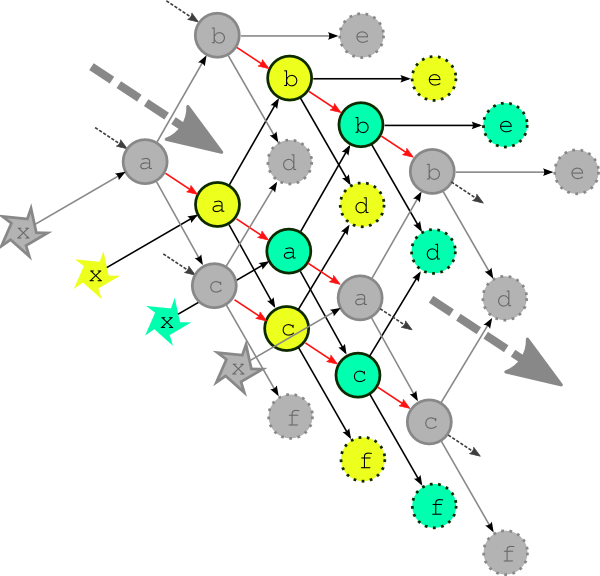
\includegraphics[width=8cm]{inkscape-svg/dep-multi-cycle} 
    \end{center}
    \caption{\small Complete dependency graph for the example
    system, assuming the least possible intercycle dependence: the
    forecast models ($a$, $b$, and $c$) depend on their own previous
    instances. The dashed arrows show connections to previous and
    subsequent forecast cycles.} 
\end{figure}



Figure~\ref{fig-time-three} shows the effect of an operational delay of
almost one whole cycle on a sequentially cycling system that has little
downtime between cycles - it takes many cycles to catch up. Above the
time axis is the optimal schedule that is possible, in principle, when
intercycle dependencies are taken into account: the second cycle after
the delay is hardly affected, and subsequent cycles are all on time.
Note that simply overlapping the single cycle schedules of 
Figure~\ref{fig-time-one} from the same start point would have resulted in
dependency violation by task {\em c}. Similarly,
Figure~\ref{fig-time-two} shows job schedules for the example system in
case study mode, or when catching up after a very long delay, when the
external driving data are available many cycles in advance.  Task {\em
a}, which as the most upstream forecast model is likely to be a resource
intensive atmosphere or ocean model, has no dependence on cotemporal
tasks and can therefore run continuously, regardless of how much
downstream processing is yet to be completed in its own, or any
previous, forecast cycle. In practice task {\em a} would depend on
cotemporal upstream tasks that wait on the external driving data, but
they would return immediately when the external data is available in
advance, so the result stands. Other tasks can cycle at regular short
intervals, the interval depending on [CHECK THIS] the task run length
relative to that of its longest cotemporal upstream dependency path. In
this case {\em c} can also run continuously, and consecutive instances
of {\em e}, which has no previous-instance dependence, can overlap.
Thus, even for this very simple example system, tasks from three or four
different cycles can in principle run simultaneously at any given
time. 

\subsection{The Cylc Scheduling Algorithm} 
\label{TheCylcSchedulingAlgorithm}

\begin{figure} \label{fig-time-two}
    \begin{center} 
        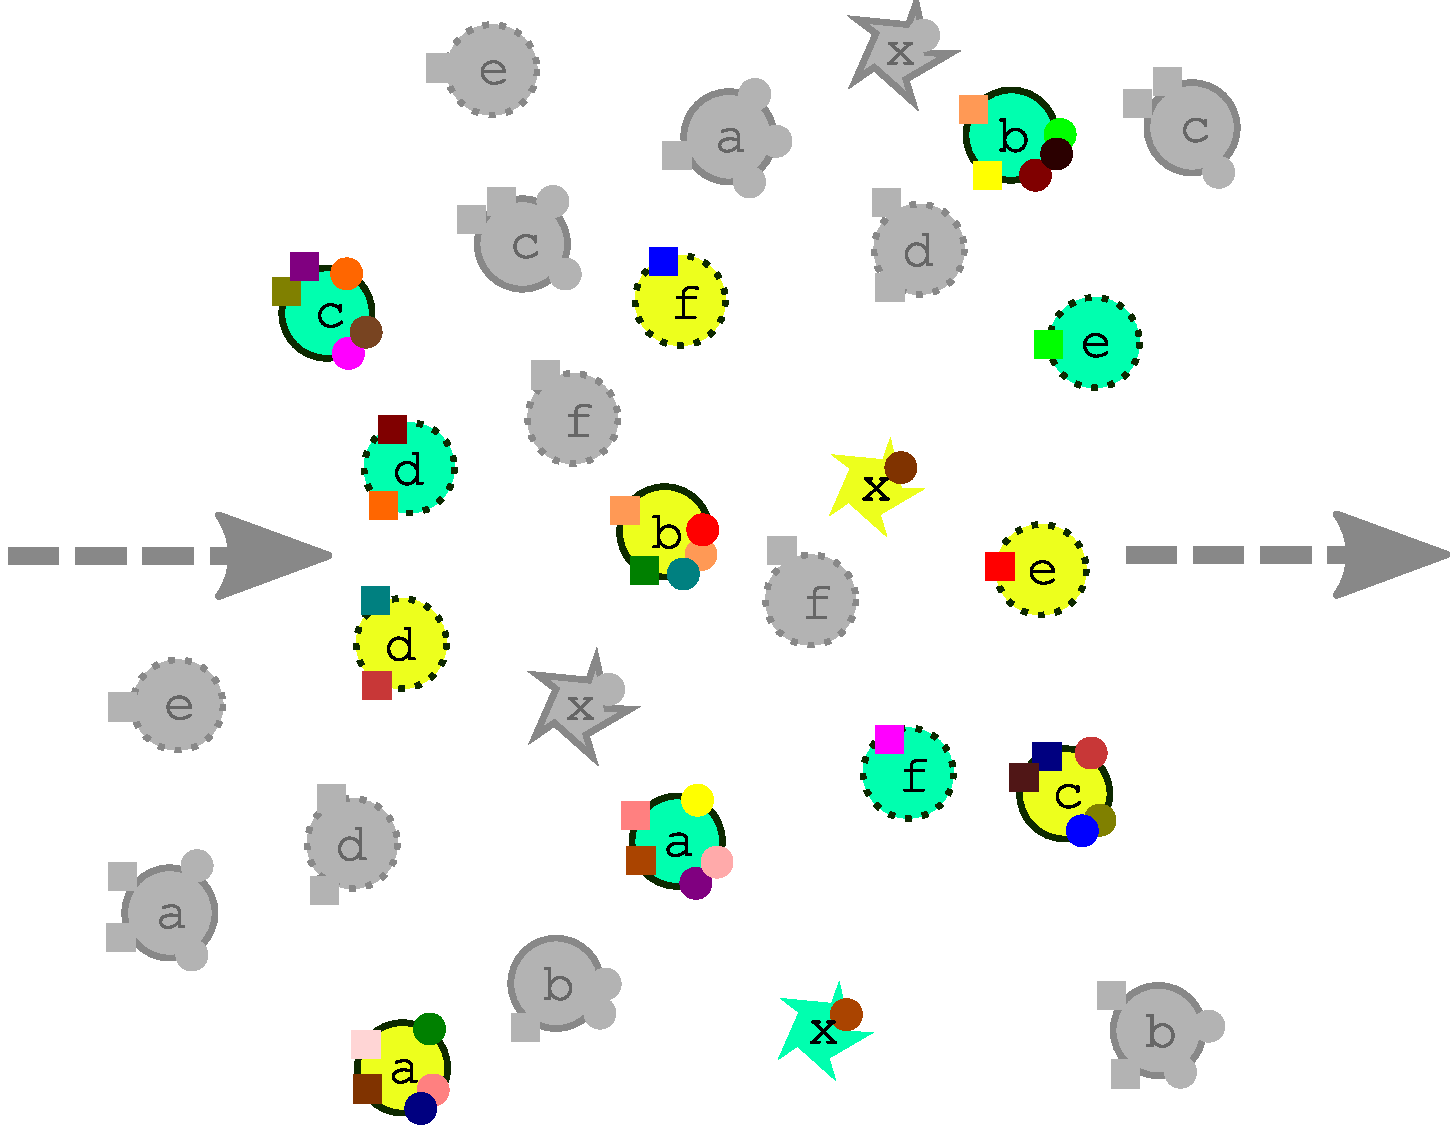
\includegraphics[width=8cm]{inkscape-svg/task-pool}
    \end{center} 
    \caption{\small How cylc sees the task pool, in contrast to the 
    full dependency diagram of Figure~\ref{fig-full}.} 
\end{figure} 

\begin{figure} \label{fig-optimal-two}
    \begin{center}
        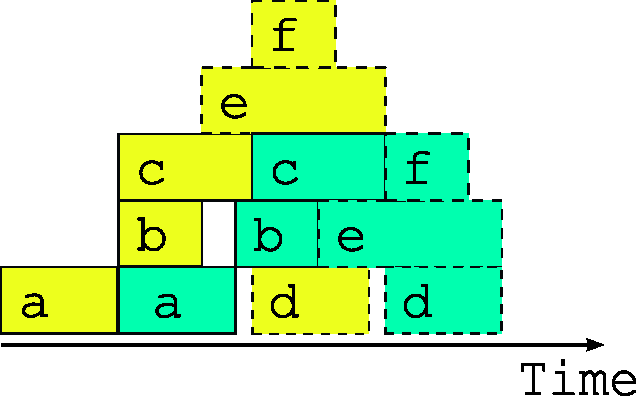
\includegraphics[width=6cm]{inkscape-svg/timeline-two-cycles-optimal} 
    \end{center}
    \caption{\small Optimal job schedule when the next cycle's driving
    data is available in advance, possible in principle when all
    intercycle dependencies are respected.} 
\end{figure} 

\begin{figure} \label{fig-time-three}
    \begin{center}
        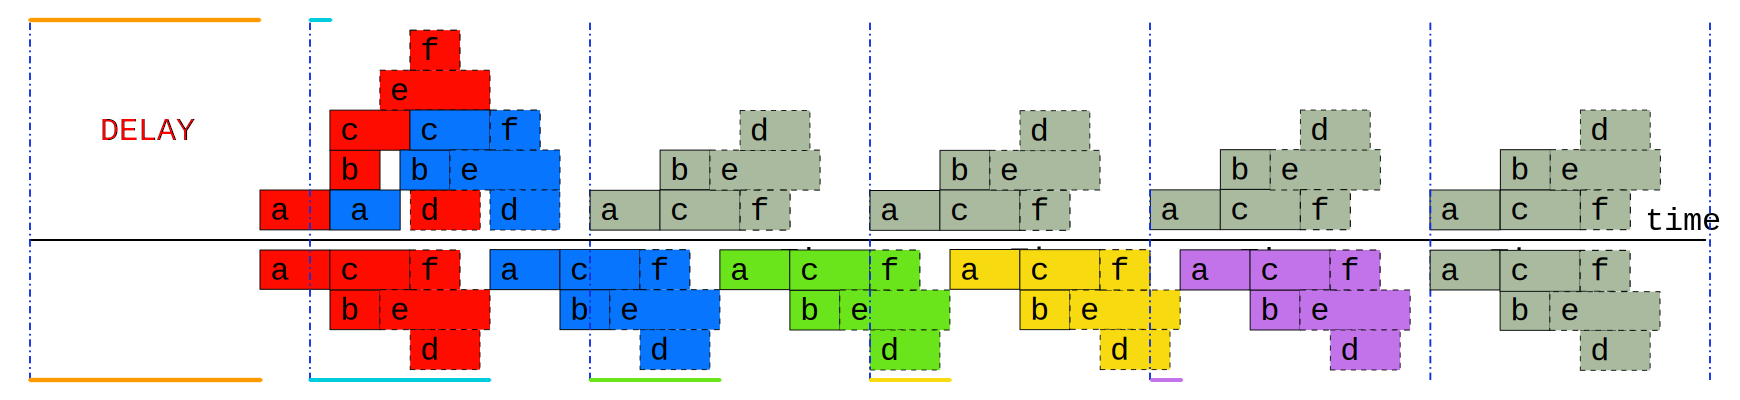
\includegraphics[width=12cm]{inkscape-svg/timeline-three} 
    \end{center}
    \caption{\small Job schedules for the example system after a delay
    of almost one whole forecast cycle, when intercycle dependencies are
    taken into account (above the time axis), and when they are not
    (below the time time axis). The colored lines indicate the time that
    each cycle is delayed, and normal ``caught up'' cycles
    are shaded gray.} 
\end{figure} 

\begin{figure} \label{fig-time-two}
    \begin{center} 
        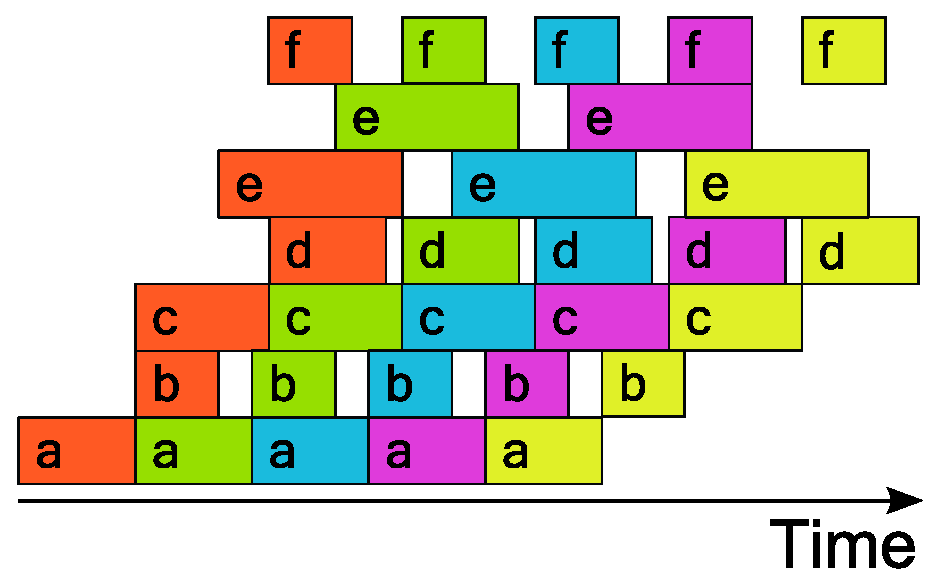
\includegraphics[width=8cm]{inkscape-svg/timeline-two}
    \end{center} 
    \caption{\small Job schedules for the example system in case study
    mode, or after a long delay, when the external driving data are
    available many cycles in advance. Above the time axis is the optimal
    schedule obtained when the system is constrained only by its true
    dependencies, as in Figure \ref{fig-dep-two}, and underneath is
    the best that can be done, in general, when intercycle dependencies
    are ignored.} 
\end{figure} 

Cylc manages a pool of proxy objects that represent real tasks in the
forecasting system. There is no global cycling mechanism to advance the
system in time; instead each individual task proxy has a private cycle
time and spawns its own successor at the right time (which depends only
on the task proxy's own type and state, not on the state of other task
proxies in the system; see Section~\ref{tasktypes}). Task proxies
are self-contained and do not know what other tasks exist in the system,
they just know their own prerequisites and outputs.  Prerequisites can
include files (say) that happen to be generated by other tasks with
different cycle times, and the task pool can contain proxies with many
different cycle times.  Now, whenever any task proxy changes state (as a
result of an output completion message, for example) cylc gets the
entire pool to interact indiscriminately, {\em regardless of cycle
times}, in an attempt to match unsatisfied prerequisites with completed
outputs.\footnote{In fact this dependency negotiation goes through a
middleman or broker object, which reduces the interaction scaling
from $n^2$ to $n$, where $n$ is the number of task proxies.} Finally, a
task proxy object can run its real task when its prerequisites are
satisfied and, by means of a messaging system, can record completion of
its own outputs as the system runs. 

Thus without using global cycling mechanisms, and treating all
dependencies equally, cylc in effect gets a set of tasks to
self-schedule by negotiating its own dependencies: optimal scheduling,
as illustrated in the previous section, emerges naturally at run time.
In addition, cylc does not distinguish between delayed and real time
operation at all. In delayed operation the tasks that gather the
system's external driving data will return immediately (because the data
is already available) and the system will only be constrained by its
internal dependencies. In real time operation, the data gathering tasks
will return only when the external data becomes available (normally at
some known time interval after the task's nominal cycle time), delaying
downstream tasks until then, by which time the previous forecast cycle
will have completed. A cylc system thus transitions seamlessly from
optimal multicycle scheduling to ``normal'' distinct forecast cycles as
it catches up to real time operation.

Note that in addition to achieving optimal scheduling, this algorithm is
extremely simple. The operator does not have to specify order of
execution or system dependencies (except implicitly, in that each task's
prerequisites must be matched by someone's outputs). The entire
forecasting system is defined by a simple list of tasks each of which,
in effect, thinks it is alone in the world (even a standalone task must
know its own prerequisites and outputs).\footnote{You can still use
explicit task dependence if you wish: just make a task depend on an
explicitly named upstream supplier {\em finishing} rather than on the
upstream output that is the actual prerequisite of interest. However,
framing prerequisites in terms of required input filenames, or similar,
results in a more flexible system: tasks can easily be ``hot replaced''
by other tasks that generate similar outputs for instance.}  For this to
work, of course, the life cycle of a task proxy object must be such that
it is guaranteed to exist by the time it is needed, but not too much
earlier, and it should die not too long after it is no longer needed.
This requires some thought at the program design stage, but the
complexities therein are entirely hidden from the user. 

\subsection{Comparison with Existing Schedulers} 
\label{ComparisonwithExistingSchedulers}

As explained earlier, as far as the author is aware current forecast
schedulers ignore intercycle dependencies and therefore require
strict sequential cycling, which is very much sub-optimal outside of
normal real time operation. The simplest of these schedulers places the
burden of scheduling almost entirely on the user, who must supply a list
of tasks that the system will run through in order, perhaps with some
way of manually specifying crude functional parallelism.  This is
clearly sub-optimal even for quite simple systems and strict sequential
cycling, and task ordering has to be re-evaluated manually whenever the
system is changed. 

Another approach is hardwired system-specific finite state scheduling
logic that enforces a predetermined order of events: {\em if tasks A and
B have finished, then start task C} and so on. Optimal scheduling within
a forecast cycle is possible in this case, assuming correct coding, but
the hard coded logic inevitably becomes convoluted and inflexible as
system complexity increases, and handling to intercycle dependencies is
almost certainly not feasible.  

Finally, the well established SMS system from ECMWF is an industrial
strength general scheduling tool for dependent jobs. Users define ``SMS
suites'' that group tasks into ``families'' and define explicit
dependency relationships between tasks and/or/? families. SMS does not
appear to be able to do optimal cycle-independent scheduling, however,
or at least is not able to do so when configured for normal usage (THIS
IS STILL NOT ENTIRELY RESOLVED!) because (a) whole families trigger 
at once(?), rather than individual tasks, and global cycling mechanisms
are used to advance the system forward in time (either looping
over successive analysis times for ``catch up'' OR triggering off the
wall clock for real time operation. Thus, in contrast to cylc, it would
not be possible to have a delayed parallel test system catch up to the
main operation and then keep pace with it.

%In other words the task pool must include waiting tasks whose
%prerequisites may {\em soon} be satisfied (but preferably no waiting
%tasks whose prerequisites will not be satisfied for some time yet),
%tasks that are currently running, and finished tasks whose outputs
%could still be needed by any current or future waiting task (but
%preferably not any finished tasks whose output will no longer be needed
%by anyone). 



\pagebreak
\section{Installing Cylc} 
\label{InstallingCylc}

\subsection{System Requirements} 
\label{SystemRequirements}

\begin{itemize}
    \item A Unix or Linux operating system
    \item The Python programming language
    \item Pyro (Python Remote Objects)
\end{itemize}

Cylc has been tested with Python 2.6, and Pyro 3.9 and 3.10,
but it should work with any recent versions of Python 2 and Pyro.
As yet neither cylc nor Pyro are compatible with Python 3. 

\subsection{Getting Cylc} 
\label{GettingCylc}

See Section~\ref{pyro} for how to get Pyro.

Cylc is currently maintained using {\em darcs}, a distributed revision
control system. If you need to develop cylc you can request access to
clone the central repository, otherwise you will receive a cylc
distribution tarball. 

\subsection{Installation} 
\label{Installation}

Pyro comes with simple installation instructions (it installs into the
standard Python modules path). 

Cylc is designed to be installed into a normal user account: simply
unpack the tarball, or move the repository, to the location of your
choice. There is no ``build'' required because cylc is written in Python
(plus a few small bash scripts).

\subsection{Environment} 
\label{Environment}

The cylc bin directory must be in your executable search path, to
provide access to cylc commands, and the cylc source directory must be
in your Python module search path, to provide access to the cylc core
modules. For sh-style login shells add the following to
your \lstinline=$HOME/.profile=:

\lstset{language=bash} 

\begin{lstlisting}
    # provide access to the cylc scheduler
    CYLC_DIR=####PATH-TO-TOP-LEVEL-CYLC-INSTALL-DIR####
    export PATH=$CYLC_DIR/bin:$PATH
    export PYTHONPATH=$CYLC_DIR/src:$PYTHONPATH
\end{lstlisting}

\subsection{Testing} 
\label{Testing}

Test the new installation by running the packaged example systems
(Section~\ref{examples}). These should work ``out of the box'', in
dummy mode or real mode, but refer to the rest of this document, and/or
\lstinline=cylc help= for more information.  

Configure the example system, register it for use, and run it:

\begin{lstlisting}
    cylc configure $CYLC_DIR/sys/examples/userguide

    cylc register userguide $CYLC_DIR/sys/examples/userguide

    cylc schedule --start-at=2010102318 userguide
\end{lstlisting}

In another terminal window open a monitor to view the running system:

\begin{lstlisting}
    cylc monitor -a userguide
\end{lstlisting}

In yet another terminal, shut the system down by remote control,
the restart it:

\begin{lstlisting}
    cylc stop userguide
    cylc start -r userguide
\end{lstlisting}

\pagebreak
\section{System Definition} 
\label{SystemDefinition}

Cylc sees a forecasting system as an evolving pool of {\bf tasks}
with clearly defined {\bf prerequisites} and {\bf outputs}
(Section~\ref{PrerequisitesAndOutputs}), where {\bf a task
is any group of one or more processes treated as a single entity for
scheduling purposes}.


\subsection{System Granularity} 
\label{System Granularity}

A system can contain a small number of large, internally complex tasks;
a large number of small, simple tasks; or anything in between. However,
because cylc can handle large systems and is entirely self organising
there are advantages to the fine-grained approach: 

\begin{itemize}
    \item better ``functional parallelism'' (multiple tasks running
        at the same time whereever possible).
    \item a more modular and transparent system.
    \item faster recovery from failures - rerun just the tasks(s) that
        failed. 
    \item the same external task script (e.g.\ for moving files around)
        can often be invoked, with different arguments, for multiple
        tasks.
\end{itemize}

\subsection{Task Behaviour} 
\label{Task Behaviour}

Make sure your system tasks behave as suggested below in order to get
the most out of cylc, and to avoid certain dire situations that are by
no means specific to cylc.

\subsubsection{Tasks Should Be Restartable}

If a particular task dies for any reason it will appear as 'failed' in
the cylc monitor and will hold up any dependant tasks downstream of it.
Once the problem is fixed the system operator can tell cylc to reset
the task, which will result in it being resubmitted at the same cycle
time. Alternatively, if the entire system is restarted after being shut
down, any task listed as 'failed' at shutdown will be resubmitted
with the same cycle time (although you can edit the system state dump
file to change this behaviour - see Section~\ref{xxx}). 

Therefore it should be possible to rerun any failed task by simply
resubmitting it for the same cycle time. 


\subsubsection{Successive Instances Of A Task Should Not Interfere}

The next instance of any task (i.e.\ the same task in the next forecast
cycle) should be able to start running as soon as its prerequisites
are all satisfied {\em even if its predecessor is not finished yet}. This
means that several instances of a post processing task, which would not
normally have any previous instance dependence, should be able to run
entirely in parallel, and a forecast model should be able to start as
soon its previous-instance restart prerequisite is satisfied even if 
the previous instance is still running (assuming, in both cases, that all 
other prerequisites are satisfied and sufficient computational resource
is available). 

If this is not the case for any particular task (perhaps because of
potential conflicts in the use of temporary files, for instance) then
cylc can force the task to run sequentially, but the resulting system
will clearly be less efficient than it could be.


\subsubsection{Tasks Should be Multicycle Restartable}

Any task that writes "intermediate files" or "restart files" that are
used by the same task in the forecast next cycle should organise these
file by cycle time (via file or directory naming conventions) so that
the same files are not simply overwritten each time. Otherwise
accidental invocation of the task for the wrong cycle time may corrupt
the intermediate files and make it impossible to go back and run the
correct cycle, thereby necessitating a cold start rather than continued
warm cycling. You may need to be aware of this in the case of monolithic
"forecast model" tasks that should really be split into multiple tasks
(imagine a monolithic "weather forecast" task that encompasses obs
processing, data assimilation, and the actual forecast model, each
part of which writes output files that are used as input by the next
part). 


\section{Quick Start Guide} 
\label{QuickStartGuide}

The following is a quick summary of the steps required to get a system
running under cylc. 

\subsection{Constructing A New Forecasting System}

You can get the {\em scheduling} right for a complex system without ever
having to run real tasks, but testing incrementally in dummy mode as you
define each task. Then (or in parallel with the task definition process)
you can also test the real system incrementally as you write its task
scripts (by which cylc runs the real tasks) by turning off all the
tasks that you're not yet interested in (this can be done through the
'--include' and '--exclude' scheduler options, or by commenting tasks
out of the configured task list.

\pagebreak
\subsection{System Definition} 

\begin{itemize}
    \item divide a system into {\bf tasks} with defined {\bf
        prerequisites} and {\bf outputs} (Section~\ref{tasks}).

    \item write a {\bf task definition file} for each task
        (Section~\ref{taskdefs}).

    \item write {\bf task scripts} to run the external tasks
        (Section~\ref{taskscripts}).
\end{itemize}

\subsection{System Configuration}
\label{QuickSystemConfiguration}

To generate task class and config modules for a system defined in
location PATH (Section~\ref{configure}): 

\begin{lstlisting}
    cylc configure [options] PATH
\end{lstlisting}

Customise the config file if necessary, and reconfigure the system
whenever task definition files are added, removed, or modified.

\subsection{System Registration}

Registration associates a name with a system definition directory. You
can then run, monitor, and control the registered system by name. The
\lstinline=register= command also has options for managing your system
registrations (checking their validiy, deleting them, and so on).

\begin{lstlisting}
    cylc register -s SYSTEM PATH
\end{lstlisting}

Where PATH is the location of the system definition directory, and SYSTEM
is the name by which you want to access the system. 

\subsection{Starting A Pyro Nameserver}

If you do not already have a Pyro nameserver running
(Section~\ref{pyro}), start one with \lstinline{nohup} so that it will
not die with your terminal session: 

\begin{lstlisting}
    nohup pyro-ns &
\end{lstlisting}

\subsection{Running And Manipulating A Registered System}

For the quick guide to starting up, manipulating, monitoring,
interrogating, pausing, resuming, or shutting down a running system,
refer to cylc command self-documentation:

%\begin{lstlisting}
%    cylc --help
%    cylc COMMAND --help
%\end{lstlisting}
    
Command usage output is also listed in the Command Reference,
Section~\ref{CommandReference}.

\pagebreak
\subsection{The System Definition Directory} 
\label{TheSystemDefinitionDirectory}

Every forecasting system to be run by cylc needs a system definition
directory containing: 

\begin{itemize} 
    \item a \lstinline=taskdef= sub-directory for your task definition
        files.
    \item a \lstinline=scripts= sub-directory for your system scripts.
\end{itemize} 

In addition, when you run \lstinline{cylc configure}, task class and
config modules will be generated and written into the system directory.
Here's the system definition directory for one of cylc's example
systems: 

\lstset{language=bash}
\begin{lstlisting}
$CYLC_DIR/sys/examples/userguide/
   system_tasks.py     # AUTOGENERATED by 'cylc configure' 
   config_defaults.py  # AUTOGENERATED by 'cylc configure' 
   config_override.py  # customizable config (autogenerated once) 
   taskdef/            # task definition files, e.g.:
      A.def              # defines task A
      B.def              # defines task B
      ...
   scripts/            # task scripts, e.g.:
      A.sh               # called by cylc to execute task A
      B.sh               # called by cylc to execute task B
      ...
\end{lstlisting}

\subsubsection{Code Management}

Several simple example systems are maintained in the cylc source
repository.  Other systems should be maintained elsewhere in their
own version control repository, with tags indicating compatibility with
particular versions of cylc.

\subsubsection{Location}

Cylc's example systems are located under \lstinline=[CYLC_DIR]/sys=.
Other systems, as explained above, should be maintained in another
location, but for ease of use they can be symlinked into the cylc system
directory.



\section{Task Definition Files} 
\label{TaskDefinitionFiles}

A simple {\bf Task Definition File} must be written for each task.
\lstinline=cylc configure= parses these and generates a Python module
that defines the task proxy classes for the system. {\bf Task
Definition Files define just the properties of tasks that matter from a
scheduling perspective: name, external task, valid cycle times,
prerequisites, outputs.} 

Other task-specific configuration settings that are not relevant to
scheduling (e.g.\ numerical method choices, MPP
domain decomposition, input and output directory locations, and so on)
belong in the external location where the real task resides, or possibly
in the cylc task scripts that run the external tasks (ideally these
should contain configuration details specific to running an external
task within the wider system, but there's nothing to stop you putting
more than that in them). However, there is one minor exception to this
rule. If your system has several tasks that essentially do the same
thing you can get them all to invoke the same external program with
task-specific input parameters supplied through environment variables
that are specified in the Task Definition Files. Forecasting systems
commonly have to move a lot of files around (from the output
directory(s) of one task to the input directory(s) of others, for
instance). See Section~\ref{RealDependencies}, and cylc's file-transfer
example in userguide !TO DO!. 

\subsection{Examples}

Listed immediately below are two example task definitions, one for a
``forecast model'', and the other not (e.g. post processing). All tasks
in a typical forecasting system can be defined as simply as these
(advanced TopNet scheduling the only exception in EcoConnect). 
But see (Section~\ref{TaskDefinitionReference}) for full Task Definition
documentation. Please refer also to the task definitions in the packaged
example systems, which show the effect of the task type modifiers as well
(particularly oneoff and contact, which will be required to some extent
in all systems).


\subsubsection{Free Task Example}

The following listing shows an example task definition for a
typical non-forecast-model task.
\lstset{language=cylctaskdef}

{
\lstinputlisting{../sys/examples/userguide/taskdef/D.def}
}

\subsubsection{Forecast Model Example}

The following listing shows an example task definition for a
typical forecast-model task.

\lstset{language=cylctaskdef}

{
\lstinputlisting{../sys/examples/userguide/taskdef/A.def}
}


\subsection{Task Types} 

Every task has to declare a {\bf Task Type}. Cylc has two basic types,
and several modifiers that change the basic type behaviour to some
extent.  

A cylc system advances by means of each individual task spawning a 
successor of the same type, at the next cycle time valid for that task,
at the right time according to its type.

\begin{itemize} \item A \lstinline=free_task= does not depend on any
        output generated by a previous instance of itself, which means
        successive instances can run in parallel, or at least overlap,
        if the opportunity arises. To allow this to happen, a free task
        spawns a successor as soon as it enters the 'running'
        state\footnote{Spawning any earlier than this would bring no
        advantage, in terms of parallel execution, at the cost of
        unrestrained breeding.}. Most non-forecast model tasks (pre and
        post processing tasks, etc.) will be of this type.

    \item A \lstinline=forecast_model= task does depend on outputs
        generated by a previous instance, namely the ``restart''
        files typically required by warm-cycling forecast models:
        each forecast is initialized in part with a ``model
        background'' generated by a recent previous forecast.
        In other words, even if all other inputs are available 
        in advance, a forecast model cannot start up until its
        restart inputs have been completed by a previous forecast
        (usually, but not necessarily, the most recent previous
        forecast). In catchup or casestudy scanarios cylc can run
        successive forecast models as soon the next restart files
        are complete, IF restart output are reported as soon as they are
        generated. In reality, however, forecast models are likely
        to run in sequence at best because (i) they tend to be large
        resource intensive models and there may not be room to run
        several at once, and (2) unless the external model itself 
        is modified to report restart outputs immediately, all 
        restart outputs will be reported complete at once when the
        model run completes.
%    # *(2) A FORECAST_MODEL depends on a previous instance of the same
%    # task to provide special 'restart' prerequisites: during a
%%    # forecast, a warm-cycling model will write out a state dump valid
%    # at the start time of the next forecast, for use in initialising
%    # it. Multiple restart outputs may be generated to allow one or more
%    # subsequent forecasts to be omitted if necessary. A forecast_model
%    # registers how many of these are generated, which cylc assumes are
%    # intended for use by the next N valid start times for the task and
%    # automatically adds special outputs and prerequisites to represent
%    # them in the system. 
%    # A forecast model cannot start running until
%    # its restart prerequisite is satisfied, but the same prerequisite
%    # can potentially be satisfied by a restart output from any of the
%    # previous N forecasts. This allows cylc to continue running when
%    # one or more cycles of a particular model have to be omitted
%    # because of problems. But in normal operation we only want a model
%    # to trigger off the most recent previous forecast, which means that
%    # a forecast model cannot spawn a successor until its *last* restart
%    # output is completed (otherwise there is a chance the next-plus-one
%    # instance could come into existence and trigger before the the
%    # current instance, and so on, in normal operation). 
 
\end{itemize}


\subsection{Task Type Modifiers} 

\begin{itemize}
    \item A \lstinline=oneoff= task never spawns a successor. Use this for 
        'cold start' tasks that supply initial inputs for starting a
        system from scratch.  See also the
        \lstinline=STARTUP_PREREQUISITES=
        task definition key, below.

    \item A \lstinline=sequential= task does not spawn a successor until it is
        finished. You can use this to force successive instances of a
        free task to run in sequence if instances of the external task
        can not be allowed to run at the same time (perhaps because they
        would interfere with each other through use of the same
        temporary files, or similar).

    \item A \lstinline=contact= task waits on an external event, such as
        incoming external data, i.e. it "makes contact" with the
        external world.  The event is expected at some defined time
        interval after the task cycle time (e.g. observational data
        might come 3.5 hours after its nominal validity time); see
        %CONTACT_DELAY below. In real time operation a contact task will
        not begin running until the clock time has reached this delayed
        start time. In catchup operation a contact task will begin
        running immediately (other prerequisites allowing) because the
        delayed start time has already passed.  
        
    \item A \lstinline=cacthup_contact= task maintains awareness,
        through a class variable (i.e. not per instance), of whether or
        not it has 'caught up' yet.  This can be used for rare occasions
        when some dependant task needs to behave differently according
        to whether its upstream contact task has caught up or not.

    \item A \lstinline=dummy= task always uses the cylc dummy task
        program for its external task, even when operating in real mode.
        The dummy task program masquerades as the task it represents by
        reporting its outputs completed at the right time. This can be
        used to provide 'fake' cold start prerequisites to get the
        system running when the real inputs have been put in place by
        some external means prior to starting up cylc.

\end{itemize}

\pagebreak
\subsection{Prerequisites and Outputs} 
\label{PrerequisitesandOutputs}

%Cylc's scheduling algorithm works by matching one task's unsatisfied
%prerequisites with another's completed outputs (Section~\ref{algorithm}). 

This sections explains how prerequisites and outputs are expressed in
cylc, and how to register them in task definition files.

\subsubsection{Interpretation As Messages} 

\begin{shaded}
    Prerequisites and outputs are literal text strings, representing
    events that are important to scheduling, sent from running tasks
    to the  task proxy objects that represent them inside cylc.
\end{shaded}

A task proxy considers a registered {\bf output} ``completed'' if it has
received a matching message from its external task.

A task proxy considers a registered {\bf prerequisite} ``satisfied'' if
any other task in the system has reported to it a matching completed
output.

For example, the message ``storm surge forecast products ready for
2009102018'' could be registered as an output by the task that generates
the referenced storm surge forecast products, and as a prerequisite by
any tasks that require them as input. 

Prerequisites and outputs typically refer to the completion of a file
or a group of files, but any event can be used: database interactions,
download from a network, copying, archiving, etc., can also be
used to trigger other tasks.

\subsubsection{The Truth Of Messages}

For an output that corresponds directly to a single file you can, if
you want, put the filename itself in the output message:
\begin{lstinline}
    "file surface-pressure-\$(CYLC_TIME).nc ready"
\end{lstinline}

However, there is no particular need to use the actual filename, 
so you might as well use a more form in order to be consistent with
messages refering to a whole group of files or other non-file-related
events:
\begin{lstinline}
    "surface pressure fields ready for \$(CYLC_TIME)"
\end{lstinline}

In particular, there is no need to include actual file locations because
cylc does not check that incoming messages (i.e.\ reports of completed
outputs) are actually true before allowing them to be used to satisfy
the prerequisites of other tasks. There are two reasons for this.
Firstly, cylc does not restrict the kind of event that can be reported
as an output (i.e. that can be used to trigger other tasks) so it would
be next to impossible for it to verify outputs in general. Secondly, 
there is no need for cylc to do it because the external tasks must
necessarily do the job themselves: if a task cannot run or cannot
complete because of missing input files, for example, it must report the
failure back to cylc immediately.


\subsubsection{Cycle Time in Messages}

Prerequisites and outputs should always contain a cycle time string to
distinguish the outputs from instances of the same task in different
forecast cycles. The time to use in messages would normally be the
task's own cycle time, since intercycle dependencies (other than
forecast model restart dependences) are rare, however cylc's task
definition mechanism (below) provides some simple cycle time arithmetic
operations for unusual cases. 

\lstset{language=Python}
\begin{lstlisting}
# example: completion of a file with date-stamped filename
"file foo_$(MY_CYCLE_TIME).bar ready"
# example: other event
"archiving completed for $(MY_CYCLE_TIME)"
\end{lstlisting}


\subsubsection{General Guidelines}

\begin{itemize}

    \item Prerequisites do not need to be unique across the system:
        multiple tasks can trigger off the same event.

    \item Outputs should be unique across the system, unless you want
        all tasks that depend on a particular output to trigger off the
        first task to provide it.

\end{itemize}

\subsubsection{Timed Output Messages}

Outputs have to be registered with an {\bf estimated time of completion}.
The timing information is currently only used in dummy mode to simulate
the correct task run time, so accuracy isn't critical. In the future
it may also be used to check system progress against expected behaviour.


\subsubsection{Forecast Model Restart Messages}

\subsection{Automatic Outputs}

\subsubsection{started and finished outputs}

\lstinline=cylc configure= automatically registers special {\bf started}
and {\bf finished} outputs for every task: 

\begin{lstlisting}
    "0 min:        foo started for $(CYCLE_TIME)"
    "[run length]: foo finished for $(CYCLE_TIME)"
\end{lstlisting}

Other tasks (via their prerequisites) can trigger off these, but 
be aware that this introduces explicit dependence on specific tasks,
rather than on outputs that could be provided, in principle, by any
task, so this makes the system somewhat less flexible.

\lstinline=cycl message= has specially options so that external tasks
can send these messages automatically, without worrying about the exact
form of the restart message (this helps guard against typographic
errors).


\subsubsection{failed and completed messages}

The {\bf failed} message should be reported by external tasks, using 
\lstinline=cylc message --failed=, whenever the task fails. This is 
not an ``output'' to be registered in the taskdef file because the
completion time is unknown at best (at what point in a tasks execution
does a failure occur?) and more usually undefined (hopefully the task
will not fail). 

Finally, \lstinline=cycl message= automatically sends a special {\bf
completed} message whenever a tasks reports {\em success or failure}:
\begin{lstlisting}
    "foo completed for $(CYCLE_TIME)"
\end{lstlisting}
 
This can be useful if you want to trigger off an upstream task whether
or not it succeeded (e.g.: a data assimilation program that triggers
when a handful of separate obs processing programs have finished or
failed, where failure occurs if no obs of a particular type happen to be
available for the forecast cycle in question).

\subsubsection{restart outputs}

Task of the 'tied' type (i.e.\ forecast models) must declare, in their
task definition files, the number (and expected output times) of
'restart outputs' that they generate to satisfy the previous-instance
dependence of their successors. Cylc configure then automatically
registers special 'restart' outputs and prerequisites for the task.
For example, consider a forecast model {\em foo} that runs on a
6 hour cycle and generates restart dumps for the next 2 cycles at
approximately 5 and 10 minutes into the forecast. This task would  
(automatically, as explained) register the following prerequisite:

\begin{lstlisting}
    "foo restart files ready for $(CYCLE_TIME)"
\end{lstlisting}

and the following two outputs:

\begin{lstlisting}
    "5 min:  foo restart files ready for $(CYCLE_TIME + 6)"
    "10 min: foo restart files ready for $(CYCLE_TIME + 12)"
\end{lstlisting}

\lstinline=cylc message= also has special options for dealing with 
restart outputs, so that external tasks do not have to worry about the
exact message format. The exception to this is oneoff cold start tasks
that provide initial restart inputs for other tasks; these currently 
have to report the right restart messages, as above, explicitly.

\pagebreak
\subsection{Task Scripts}
\label{TaskScripts}

(note that several tasks may use the same script with different
arguments, e.g. for moving files around).

The 'scripts' sub-directory of a cylc system definition is a handy
central location in which to keep system-specific scripts for running
external tasks which often have an independent existence outside of the
forecasting system. Typically the ``external task'' specified in a task
definition file will be one of these scripts which, once invoked by
cylc, will itself launch the real external process(es) and handle all
cylc messaging. In that case it may not be necessary to modify the
external task for use within cylc.  That said, you can if you wish
specify an external script in the task definition file, in which case 
the external script will have to be modified to do the cylc messaging,
OR uses cylc's task wrapping mechanism, which automatically handles the
former case but sets all outputs, including internal ones, completed
only after the external script finishes.  Scripts in the scripts
sub-directory are automatically made accessible, via \$PATH, to tasks
launched by cylc. 

\subsubsection{Task Messages}

The external tasks, or the scripts that execute them, need to report
their outputs back to cylc as they run. Section~\ref{message} shows
how to add cylc messaging to tasks.  Ideally this reporting should be
done as soon as each output is completed throughout the run. This is
easy to achieve for scripted data processing tasks, for instance, but
you may not want to do it for model executables (it should be noted that
forecast models don't normally complete their major outputs until the
end of a run - except for restart outputs!). If that is the case a task
can simply report all outputs completed at once before it finishes.
Cylc in fact has a task-wrapping mechanism that does this automatically
(Section~\ref{wrapping}), allowing you schedule a set of existing
tasks without modifying them at all.  

Each external task must:

\begin{itemize}
\item report (to cylc) when the task has started
\item report when the task has finished
\item report when every other registered task output has
completed
\end{itemize}

(Technically, the `started' and `finished' messages are just
outputs too, but they are special in that every task
must have them).

In addition, tasks can optionally:

\begin{itemize}
\item report any arbitrary unregistered (i.e. non-output)
messages, for debugging, logging, or progress monitoring purposes.
\end{itemize}

All incoming messages are logged by cylc, but only output messages can
affect the state of other task objects.

Task messages don't necessarily have to originate from top level task
control scripts. It's a probably a good idea to do this if possible, but
lower level scripts that are invoked as the task runs can communicate
directly with cylc if necessary.

\subsection{Task Wrapping}
\label{TaskWrapping}

If you have a task that for some reason you cannot, or do not want to,
modify to send the startup, output, and failure or completion messages, 
you can have cylc wrap the task in a special script that does the following:

\begin{itemize}
    \item reports task startup
    \item invokes the wrapped task, and checks for success or failure
    \item if the task failed, it reports the failure. 
    \item if the task succeeded, it automatically reports all the task's
        registered outputs complete, and then reports success.
\end{itemize}

Note the assumption that successful completion of an external task
implies all registered outputs were completed by it.

If you wrap all tasks like this you can run an entire system without
modifying the tasks at all to accommodate cylc. There is a downside to
task wrapping, however:

\begin{itemize}
    \item you can't add extra internal messages (i.e. additional to the
        registered outputs) to a task, for progress monitoring or
        debugging purposes.
    \item all registered task outputs are reported complete only
        when the wrapped task finishes, not at the time they are actually
        completed. This means successive instances of a `tied' (forecast
        model) task cannot run in parallel, or overlap, if the
        opportunity arises (because the restart outputs, which are
        normally created early in the forecast, won't be reported until
        the end of the forecast).
\end{itemize} 

Of course forecast models are usually monolithic executables that are not
well suited to spawing external messaging processes, so these problems
may be of no consequence in practice.

\pagebreak

\subsection{Handling Real Dependencies}
\label{HandlingRealDependencies}

Cylc's prerequisite and output messages are somewhat abstract, but the
fact remains that most of the time they correspond directly to real 
files (or groups of files) that are generated by one task and used by
other tasks.

Each task, when considered in isolation, could in principle be
configured to use almost any location and filenaming convention for its
input and output files. But in the context of the wider forecasting
system they must all work together, so the question arises, {\em how do
we ensure that tasks always know where to find their input files, and
should the scheduling system have anything to do with this?} 

There are several ways of dealing with this in cylc (in fact they can
be mixed and matched as you wish). 

\subsubsection{Standard Method}

The standard way of doing this is to configure the external tasks with
some knowledge of their role in the full system: each task knows where
to look for its input files because it knows where they come from,
and/or it knows where to put its output files because it knows who is
going to use them. Doing this by means of a system-wide convention for 
input and output directories  etc. for the major tasks (principally the
scientific models) makes it easy to know where files should end up at
all times (e.g. model X's output goes in /oper/X/output, for any model
X).

In this case, cylc task proxies (via their task definition files) do not
need to know anything about input and output file locations. If a task's
prerequisites are satisfied it automatically implies that the
corresponding input files exist AND are in the right location for
immediate use.

\subsubsection{Alternative Method 1}

Large scientific models typically have their own idiosyncratic
configuration defaults. You could leave each model configured in its own
``natural'' way, as if unaware of the wider forecasting system, and then
add additional ``connector'' tasks to move files around as needed
(e.g. to transfer files from X's output directory to Y's input directory).

To do this in cylc, you can either:

\begin{itemize}
    \item have a separate task script for every connector task, with the
        relevant locations hardwired into them; in this case the task
        definition files still do not need to know the locations.
    \item OR have all connector tasks call the same generic ``file
        transfer'' task script, in which the directory locations can be
        specified as environment variables in the connector task
        definition files (and the generic transfer script should be read
        them from the environment).
\end{itemize}

\subsubsection{Alternative Method 2}

Configure the external tasks to set their input and output
directories/filenames {\em dynamically} according to input taken from
environment variables, and then define these variables 
in the cylc task scripts OR task definition files. You should
(obviously) make sure, in the cylc system definition, that the various 
input and output directories are used consistently throughout the system. 
This method requires no additional connector tasks AND you don't have to
configure the external tasks with knowledge of the wider system - all of 
that comes through the cylc system definition. 

%\subsubsection{Alternative Method 3}
%
%Finally, in principle extra information could be attached to cylc output
%messages so that actual file locations could be passed dynamically from
%to whichever tasks use the output. Cylc currently cannot do this (you
%can put actual file locations in the messages, but the receiver has to
%have the exact matching message and therefore would have to know the
%location in advance). This is a possible future development, but is 
%probably not worth the effort because configuring the external tasks 
%to report this information takes more effort than putting the same
%information into the cycl task definition files. The cylc setup
%would remain entirely context-independent, which is nice, and would
%automatically pass on changes to the external input / output config of
%the system.



\section{System Configuration}
\label{SystemConfiguration}

\subsection{System Config Files}
\label{SystemConfigFiles}

Each task set to be scheduled by cylc requires a {\bf config file} that
specifies parameters such as the logging directory path, task groups,
and so on. The config file is generated automatically by 
\lstinline=cylc configure= the first time the system's task definition
files are parsed. Subsequent reconfiguration will not overwrite the
config file unless you force it (in which case the original will be
backed up), in case you have changed the default settings. The config
file is a Python source module, but it is simply structured and should
be easy for non-programmers to understand. 

All configurable items are stored in a single {\em dict} (a Python
associative array):

\lstset{language=Python}
\begin{lstlisting}
config[ 'item' ] = value
\end{lstlisting}

\subsection{Configurable Items}
\label{ConfigurableItems}

\begin{itemize} 
    
        \begin{lstlisting}
config['system_name'] = 'foo'
        \end{lstlisting}

    \item {\bf task list}: list the name of each task to instantiate at
        system startup.  For testing and debugging you can turn off
        specific tasks by simply commenting them out of the task list.
        
        \begin{lstlisting}
config['task_list'] = \
    [
        'foo',
        #'bar',
        'baz'
    ]
        \end{lstlisting}


    \item {\bf task groups}: you can group several related tasks under a
        single name for easy dynamic insertion of multiple tasks at
        once into a running system. For example, you could define a 
        group to hold all the tasks needed to cold start a particular
        model.

        \begin{lstlisting}
config['task_groups']['foo'] = [ 'bar', 'baz', ...]
        \end{lstlisting}

    \item {\bf job launch method}: the method by which cylc should
        invoke the real external tasks when their prerequisites are
        satisfied. Current methods are
        \begin{itemize}
            \item {\bf qsub}: sudo submit to a named queue as the task
                owner.  
            \item {\bf not qsub}: direct background execution.
        \end{itemize}
        To add additional external launch methods (e.g.\ for other
        queueing systems) you will need to modify the 
        \lstinline{src/task_launcher.py} source module.

        \begin{lstlisting}
config['use_qsub'] = True
config['job_queue'] = 'prime'
        \end{lstlisting}

    \item {\bf state dump directory}: the location of cylc's ``state
        dump'' files (see Section~\ref{state-dump}).  You may
        specify an absolute directory path, or one relative to the
        directory in which you run cylc.
        
        \begin{lstlisting}
config['logging_dir'] = '/foo/bar/baz/state'
        \end{lstlisting}


    \item {\bf logging directory location}: 
        This items sets the location of the system's log files. You may
        specify an absolute directory path, or one relative to the
        directory in which you run cylc.

        \begin{lstlisting}
config['logging_dir'] = '/foo/bar/baz/logging'
        \end{lstlisting}

    \item {\bf logging verbosity}: Cylc's logging subsystem is based on
        the standard Python logging module (see
        Section~\ref{logging}). The 'info' level logs messages
        relevant to task execution and scheduling, while the more
        verbose 'debug' level adds messages that trace the execution of
        cylc itself.

        \begin{lstlisting}
config['logging_level'] = logging.INFO
        \end{lstlisting}

    \item {\bf environment variables}: You can export variables into the 
        environment of all external tasks that the system runs. Note that
        this can also be done, via task definition files, on a per-task
        basis.

        \begin{lstlisting}
config['environment'][ 'VARNAME1' ] = 'value1'
        \end{lstlisting}

    \item {\bf global system constraint}: if your system contains a
        subset of tasks that do not depend on other tasks in the system, 
        you can prevent these tasks from running out far ahead of the 
        rest by setting the maximum interval (with respect to cycle
        time) that the fast task is allowed to get ahead of the slowest.
        
        \begin{lstlisting}
config['max_runahead_hours'] = 24
        \end{lstlisting}

\end{itemize}


\pagebreak

\subsection{Example Config File}
\label{ExampleConfigFile}

This is the config defaults file for the ``userguide'' example system
distributed with cylc: 

\lstset{ language=Python }
{
\lstinputlisting{../sys/examples/userguide/system_config.py}
}



\lstset{language=}

\pagebreak
\section{System Registration}
\label{SystemRegistration}

{\bf system name}: the system is registered under
        this name in your cylc preferences directory. The system name is
        then used to refer to the system in cylc commands. It is also
        used as a ``groupname'' under which to register system objects 
        in the Pyro nameserver, to prevent conflicts with other systems
        that may be running at the same time.


\section{Running Systems}
\label{RunningdSystems}

\subsection{Dummy Mode} 
\label{DummyMode}

In {\em dummy mode}, \lstinline=cylc schedule -d=, in place of each real
system task cylc executes an external program that masquerades as the
real task by reporting its registered outputs complete at the appropriate
times. This is essentially indistinguishable, to cylc, from the real
thing, and is therefore a complete test of scheduling for the configured
task set. Dummy mode allows very quick testing of scheduling and failure
recovery scenarios for arbitrarily complicated task sets.

If a system (or a failure recovery operation - see
Section~\ref{FailureRecovery}) works in dummy mode, it will work in real
operation {\em if}:
\begin{itemize}
    \item the real tasks report the correct output messages (as
        registered in the task definition files).
    \item no bug has been introduced into the messaging interface
        \lstinline=cycl message=, which is not used by the dummy 
        task program - it communicates directly with the right task
        proxy object in the running scheduler.
\end{itemize}

\subsection{Incrementally Constructing New Systems} 
\label{IncrementallyConstructingNewSystems}

Start by defining tasks at the top of the single-cycle dependency graph,
and testing in dummy mode each time a new task is added. This checks
that prerequisites and outputs match correctly. When the whole system is
defined, begin writing the real task scripts in the same order, and test
in real mode with the as yet unimplemented tasks turned off (comment
them out of the task list in the system config module, or use the
scheduler command line options provided for this purpose). 

\section{Monitoring Running Systems}
\label{MonitoringRunningSystems}


\section{Controlling Running Systems}
\label{ControllingRunningSystems}

\section{A Complete Working Example}
\label{ACompleteWorkingExample}


%THIS FILE IS INCLUDED AUTOMATICALLY IN THE USERGUIDE LaTeX SOURCE
%DURING DOCUMENT PROCESSING

The packaged system defined in,

\begin{lstlisting}
[CYLC_TOP_DIR]/sys/examples/userguide/
\end{lstlisting}

is a complete working implementation of the example used to illustrate
how cylc works of in Section~\ref{HowCylcWorks}, with the dependency
diagram shown in Figure~\ref{fig-dep-two}. It can be run in real mode or
dummy mode; the result (scheduling-wise) should be essentially
identical. The task scripts invoked in real mode create zero-sized
output files with the \lstinline=touch= command, and all tasks ``read''
and ``write'' files from the one location. See the discussion in
Section~\ref{????} for how to manage input and output file locations in
a more realistic forecasting system. While this is clearly not a real
forecasting system, it has exactly the same properties as a real system
as far as scheduling is concerned.  

The Unix 'sleep' command is used to get the trivial example tasks to
execute in the right amount of time (as defined in their taskdef files).
Then, to get the real tasks to execute as quickly as their dummy mode
counterparts, the sleep time is scaled by \lstinline=$REAL_TIME_ACCEL=,
an environment variable defined in the system config module.

The system contains the following tasks:

\begin{itemize}
    \item {\bf A} - this task could be an atmospheric forecast model,
    it depends on external real time obs and its own restart file.
    \item {\bf B} - this task could be a sea state model, it depends on 
    outputs generated by A, and its own restart file.
    \item {\bf C} - this task could be a storm surge model, it depends on 
    outputs generated by A, and its own restart file.
    \item {\bf D} - this task post processes outputs generated by B and C.
    \item {\bf E} - this task post processes outputs generated by B.
    \item {\bf F} - this task post processes outputs generated by C.
    \item {\bf X} - this "external contact" task gets the obs data required
    by A, at 1 hour past its reference time. X has no prerequisites and
    therefore runs immediately, once its contact time has passed.
\end{itemize}

There are also {\bf two additional tasks}:

\begin{itemize}
    \item {\bf startup} - a oneoff task that cleans out the system
    workspace (used by all tasks for their output files, in this
    example) at startup.
    \item {\bf coldstart} - a oneoff task provides the initial restart
    prerequisites required by the forecast models (once the system
    is cycling these are provided by previous forecasts). 
\end{itemize}

{\bf Task F illustrates the use of cylc's task wrapping mechanism} for
running unmodified external tasks (i.e. task that do not know about
cylc) - see Section~\ref{TaskWrapping}. The taskdef file ENVIRONMENT key
is used to export the cycle time, in the form expected by the wrapped
external task, into the task execution environment.

The \lstinline=$NEXT_CYCLE_TIME= and \lstinline=$NEXT_NEXT_CYCLE_TIME=
variables defined in the task definition files, and read by the external
``forecast model'' scripts, are just a convenience to allow the minimalist
external tasks to avoid doing their own cycle time arithmetic to compute
the validity times of their restart outputs.

{\bf To run the example system} follow the Quick Start instructions from
the 'configure' step onward (Section~\ref{QuickSystemConfiguration}).


\lstset{ basicstyle=\color{basic}\tiny\ttfamily }

\pagebreak
\subsection{Startup Task}
\subsubsection{Definition}
\lstset{language=cylctaskdef}
\lstinputlisting{../sys/examples/userguide/taskdef/startup.def}
\subsubsection{Script}
\lstset{language=bash}
\lstinputlisting{../sys/examples/userguide/scripts/startup.sh}

\pagebreak
\subsection{Coldstart Task}
\subsubsection{Definition}
\lstset{language=cylctaskdef}
\lstinputlisting{../sys/examples/userguide/taskdef/coldstart.def}
\subsubsection{Script}
\lstset{language=bash}
\lstinputlisting{../sys/examples/userguide/scripts/coldstart.sh}

\pagebreak
\subsection{Task X}
\subsubsection{Definition}
\lstset{language=cylctaskdef}
\lstinputlisting{../sys/examples/userguide/taskdef/X.def}
\subsubsection{Script}
\lstset{language=bash}
\lstinputlisting{../sys/examples/userguide/scripts/X.sh}

\pagebreak
\subsection{Task A}
\subsubsection{Definition}
\lstset{language=cylctaskdef}
\lstinputlisting{../sys/examples/userguide/taskdef/A.def}
\subsubsection{Script}
\lstset{language=bash}
\lstinputlisting{../sys/examples/userguide/scripts/A.sh}

\pagebreak
\subsection{Task B}
\subsubsection{Definition}
\lstset{language=cylctaskdef}
\lstinputlisting{../sys/examples/userguide/taskdef/B.def}
\subsubsection{Script}
\lstset{language=bash}
\lstinputlisting{../sys/examples/userguide/scripts/B.sh}

\pagebreak
\subsection{Task C}
\subsubsection{Definition}
\lstset{language=cylctaskdef}
\lstinputlisting{../sys/examples/userguide/taskdef/C.def}
\subsubsection{Script}
\lstset{language=bash}
\lstinputlisting{../sys/examples/userguide/scripts/C.sh}

\pagebreak
\subsection{Task D}
\subsubsection{Definition}
\lstset{language=cylctaskdef}
\lstinputlisting{../sys/examples/userguide/taskdef/D.def}
\subsubsection{Script}
\lstset{language=bash}
\lstinputlisting{../sys/examples/userguide/scripts/D.sh}


\pagebreak
\subsection{Task E}
\subsubsection{Definition}
\lstset{language=cylctaskdef}
\lstinputlisting{../sys/examples/userguide/taskdef/E.def}
\subsubsection{Script}
\lstset{language=bash}
\lstinputlisting{../sys/examples/userguide/scripts/E.sh}


\pagebreak
\subsection{Task F}
\subsubsection{Definition}
\lstset{language=cylctaskdef}
\lstinputlisting{../sys/examples/userguide/taskdef/F.def}
\subsubsection{Script}
\lstset{language=bash}
\lstinputlisting{../sys/examples/userguide/scripts/F.sh}


\pagebreak
\section{Command Reference}
\label{CommandReference}

Cylc commands are intended to be largely self documenting so the
attendant text in this section is minimal: for each command there is
just reference to other relevant sections of this document.  

The listings below are actual command output generated during document
processing, to ensure that the information is completely up to date. 

\lstset{ basicstyle=\color{basic}\footnotesize\ttfamily }

\subsection{cylc}
\label{cylc}


\lstset{language=usage}

{
\lstinputlisting{command-usage/cylc-help.txt}
}

\pagebreak
\subsection{cylc configure}
\label{cylcconfigure}

See Section~\ref{configuration} for complete documentation of system
configuration.

{ 
\lstinputlisting{command-usage/cylc-configure.txt} 
}

\pagebreak
\subsection{cylc register}

See Section~\ref{registration} for complete documentation of system
registration.


{ 
\lstinputlisting{command-usage/cylc-register.txt} 
}

\pagebreak
\subsection{cylc schedule}
\label{cylcschedule}

See Section~\ref{schedule} for complete documentation of system
scheduling.

{
\lstinputlisting{command-usage/cylc-schedule.txt}
}

\pagebreak
\subsection{cylc stop}
\label{cylcstop}

{
\lstinputlisting{command-usage/cylc-stop.txt}
}

\pagebreak
\subsection{cylc pause}
\label{cylcpause}

{
\lstinputlisting{command-usage/cylc-pause.txt}
}

\pagebreak
\subsection{cylc resume}
\label{cylcresume}

{
\lstinputlisting{command-usage/cylc-resume.txt}
}

\pagebreak
\subsection{cylc set-level}
\label{cylcsetlevel}

{
\lstinputlisting{command-usage/cylc-set-level.txt}
}

\pagebreak
\subsection{cylc nudge}
\label{cylcnudge}

{
\lstinputlisting{command-usage/cylc-nudge.txt}
}

\pagebreak
\subsection{cylc task-dump}
\label{cylcask}
\lstinputlisting{command-usage/cylc-task-dump.txt}

\subsection{cylc task-what-is}
\label{cylcask}
\lstinputlisting{command-usage/cylc-what-is.txt}

\pagebreak
\subsection{cylc reset}
\label{cylcreset}

{
\lstinputlisting{command-usage/cylc-reset.txt}
}

\pagebreak
\subsection{cylc kill}
\label{cylckill}

{
\lstinputlisting{command-usage/cylc-kill.txt}
}

\pagebreak
\subsection{cylc purge}
\label{cylcpurge}

{
\lstinputlisting{command-usage/cylc-purge.txt}
}

\pagebreak
\subsection{cylc insert}
\label{cylcinsert}

{
\lstinputlisting{command-usage/cylc-insert.txt}
}

\pagebreak
\subsection{cylc message}
\label{cylcmessage}

{
\lstinputlisting{command-usage/cylc-message.txt}
}

\pagebreak
\subsection{cylc run-task}
\label{cylcruntask}

{
\lstinputlisting{command-usage/cylc-run-task.txt}
}

\pagebreak
\subsection{System Monitors}
\label{Systemmonitors}

\subsubsection{cylc monitor}
\label{cylcmonitor}
{
\lstinputlisting{command-usage/cylc-monitor.txt}
}

\pagebreak
\subsubsection{cylc monitor-r}
\label{cylcmonitor-r}
{
\lstinputlisting{command-usage/cylc-monitor-r.txt}
}

\pagebreak
\subsubsection{cylc monitor-d}
\label{cylcmonitor-d}
{
\lstinputlisting{command-usage/cylc-monitor-d.txt}
}

\subsubsection{cylc monitor-p}
\label{cylcmonitor-p}
{
\lstinputlisting{command-usage/cylc-monitor-p.txt}
}

\pagebreak
\section{Master Task Definition Template}
\label{MasterTaskDefinitionTemplate}

Listed below is the full task definitition template with all items
documented.

\lstset{language=cylctaskdef}

\lstinputlisting{../sys/templates/taskdef/master.def}

\lstset{language=}

\pagebreak
\subsection{More Complex Task Behaviour}
labelsubsection{MoreComplexTaskBehaviour}

DETAIL WHEN IS IT NECESSARY TO DERIVE PYTHON TASK CLASSES DIRECTLY
I.E. WHEN ARE CYLC TASK DEFINITION FILES NOT SUFFICIENT.
(In EcoConnect: only streamflow and topnet)

\pagebreak
\section{Master Task Script Templates}
\label{MasterTaskScriptTemplates}


See also cylc task wrapping documentation, Section~\ref{TaskWrapping},
which allows cylc to control unmodified external tasks (at the cost that
internal outputs are only reported when the task finishes).

\lstset{language=bash}

The following variables are automatically exported by cylc into
the execution environment of a each task:
\begin{itemize}
   \item \lstinline=$TASK_NAME= - what cylc calls the task (not the
       filename of the task script). 
   \item \lstinline=$CYCLE_TIME= - task-specific forecast cycle time.
   \item \lstinline=$CYLC_NS_GROUP= - Pyro nameserver group name used by the system.
   \item \lstinline=$CYLC_NS_HOST= - Pyro nameserver hostname.
\end{itemize}

When called by a task script, \lstinline=cylc message= also has access to
these variables, which enables it to communicate with the correct task
proxy object within the running scheduler. 

The only one of these variables that you should need to use explicitly
within task scripts is the cycle time, \lstinline=$CYCLE_TIME=.

Tasks may also have access to custom task-specific environment variables
set in the task definition file.

If a task script is executed manually or by \lstinline=cylc run-task=
then \lstinline=cylc message= will print to stdout instead of attempting
to communicate with a task proxy object registered in a Pyro nameserver.


\lstset{language=bash}

\pagebreak
\subsection{Free Tasks}
\lstinputlisting{../sys/templates/scripts/free-task.sh}

\pagebreak
\subsection{Tied Tasks}
\lstinputlisting{../sys/templates/scripts/tied-task.sh}

\appendix

\pagebreak
\section{Object Oriented Programming}
\label{ObjectOrientedProgramming}

Cylc relies heavily on Object Oriented Programming (OOP) concepts,
particularly the {\em polymorphic} nature of the task proxy objects.
This section gives a very minimal explanation of what this means;
please refer to an OOP reference for more detail.

A {\bf class} is a generalisation of data type to include behaviour
(i.e.\ functions or methods) as well as state. 

%For example, a $shape$ class could define a $position$ data member to
%hold the location of a shape object, a $move()$ method that by which
%a shape object can alter its position, and a $draw()$ method that
%causes it to display itself on screen.

An {\bf object} is a more or less self contained specific instance
of a class. This is analagous to specific integer variables being 
instances of the integer data type.

A {\bf derived class} or {\bf subclass} {\em inherits} the properties
(methods and data members) of its parent class. It can also override
specific properties, or add new properties that aren't present in the
parent. Calling a particular method on an object invokes the object's
own method if one is defined, otherwise the parent class is searched,
and so on down to the root of the inheritance graph. 

%For example, we could derive a $circle$ class from $shape$, adding a
%`radius' data member and overriding the $draw()$ to get circle objects
%to display themselves as actual circles.  Because we didn't override the
%$move()$ method, calling $circle.move()$ would invoke the base class
%method, $shape.move()$. 


{\bf Polymorphism} is the ability of one type to appear as and be used
like another type.  In OOP languages with inheritance, this usually
refers to the ability to treat derived/sub-class objects as if they were
members of a common base class. In particular, a group of mixed-type
objects can all be treated as members of a common base class. 
%For example, a group of %$circles$, $triangles$, and $squares$ could 
%be manipulated by code designed entirely to handel $shapes$; calling
%$[shape].draw()$ will invoke the right derived class $draw()$ method. 
This is a powerful mechanism because it allows an existing program,
without modification, to manipulate new objects so long as they 
derive from the same base class as the original objects.
%If we later derive an entirely new kind of shape ($hexagon$, say) with
%it's own unique behaviour, the existing program, without modification,
%will process the new objects in the proper hexagon-specific way.  

In cylc, all task proxy objects are derived from a base class that 
embodies the properties and behaviour common to all task proxies. 
The scheduling algorithm works with instances of the base class so that
any current or future derived task object can be handled by the program
without modification (other than deriving the new subclass itself).


\pagebreak
\section{Pyro} 
\label{Pyro}

Pyro (Python Remote Objects) is a widely used open source objected
oriented Remote Procedure Call technology, see {\em
http://pyro.sourceforge.net}.

\subsection{Pyro Software License (MIT license)}
\label{PyroSoftwareLicense(MITlicense)}

Pyro is Copyright (c) 2002  by Irmen de Jong.

Permission is hereby granted, free of charge, to any person obtaining a
copy of this software and associated documentation files (the
``Software''), to deal in the Software without restriction, including
without limitation the rights to use, copy, modify, merge, publish,
distribute, sublicense, and/or sell copies of the Software, and to
permit persons to whom the Software is furnished to do so, subject to
the following conditions:

The above copyright notice and this permission notice shall be included
in all copies or substantial portions of the Software.

THE SOFTWARE IS PROVIDED ``AS IS'', WITHOUT WARRANTY OF ANY KIND,
EXPRESS OR IMPLIED, INCLUDING BUT NOT LIMITED TO THE WARRANTIES OF
MERCHANTABILITY, FITNESS FOR A PARTICULAR PURPOSE AND NONINFRINGEMENT.
IN NO EVENT SHALL THE AUTHORS OR COPYRIGHT HOLDERS BE LIABLE FOR ANY
CLAIM, DAMAGES OR OTHER LIABILITY, WHETHER IN AN ACTION OF CONTRACT,
TORT OR OTHERWISE, ARISING FROM, OUT OF OR IN CONNECTION WITH THE
SOFTWARE OR THE USE OR OTHER DEALINGS IN THE SOFTWARE.
                                          
\subsection{Single- or Multi-Threaded Pyro?}
\label{Single-orMulti-ThreadedPyro?}

In single threaded mode Pyro's \lstinline=handleRequests()= returns
after either a timeout has occurred or at least one request
(i.e.\ remote method call) was handled. Using \lstinline|timeout = None| 
allows us to process tasks {\em only} after remote method invocations
come in.  Further, we can detect the remote calls that actually change
task states, and thereby drop into the task processing code only when
necessary, which eliminates a lot of extraneous output when debugging
the task processing loop (e.g.\ in dummy mode there are a lot of remote
calls on the dummy clock object, which does not alter tasks at all). 

In multithreaded mode, \lstinline=handleRequests()= returns immediately
after creating a new request handling thread for a single remote object,
and thereafter remote method calls on that object come in asynchronously
in the dedicated thread. This is not good for cylc's scheduling
algorithm because tasks are only set running in the task processing
block which can be delayed while \lstinline=handleRequests()= blocks waiting
for a new connection to be established, even as messages that warrant
task processing are coming in on existing connections. The only way
around this seems to be to do task processing on \lstinline=handleRequests()=
timeouts which results in a lot of unnecessary processing when nothing
important is happening.

\subsection{Running Pyro}
\label{RunningPyro}

To see if there is a Pyro nameserver running already on your network
segment, use \lstinline=pyro-nsc [-h host] [-p port]=. Invoke the
command without arguments to see a list of options.

To start a Pyro nameserver, use \lstinline{nohup} so that it
will not die with your terminal session: 

\begin{lstlisting}
    nohup pyro-ns &
\end{lstlisting}

For more detailed information, see the Pyro manual / userguide.

\pagebreak
\section{Miscellaneous Notes}
\label{MiscellaneousNotes}

\subsection{Orderly Product Generation}
\label{OrderlyProductGeneration}

Note that ``correct scheduling'' is not equivalent to ``orderly
generation of products by cycle time'' - under cylc a product
generation task will trigger as soon as its prerequisites are satisfied,
whether or not other tasks associated with the same cycle time are
running yet. If your product presentation or delivery system demands
that all products for one cycle are complete before any from the next
cycle, then (a) this is inefficient - fix it!, or (b) introduce artificial
dependencies into your system to enforce strict sequential cycling (but
that, of course, nullifies the principal advantage of using cylc in the
first place!), or (c) write a script that monitors the output from 
your cylc system and reports completion of a cycle only when the last
products associated with that cycle are complete. 

%\subsection{Catching Up}
%labelsubsection{CatchingUp}
%
%The state of being ``caught up'' or not is a property of individual
%tasks, not the whole system, and additionally it should only matter to
%external contact tasks, i.e. those that wait on external data that is
%available at a wall clock time of T (task cycle time) + o (some offset
%insterval). Where this matters an external task can detect whether or
%not it has caught up (and signal this to its proxy object in cylc) by
%comparing its cycle time (and offset) to the wall clock time.

\subsection{Running Multiple Instances Of The Same System}
\label{RunningMultipleInstancesOfTheSameSystem}

what this means - use of the exact same task and config modules, under 
different registered names.

consequences - dummy mode fine (e.g. multiple users running the standard
cylc example systems)
             - real mode: the external tasks must not interfere! Could
             use system name in all important dir paths, but prob better 
             to copy the system def directory AND invoke different versions
             of the external tasks (e.g. under /oper and /test)

    Registered names are also used along with your username to construct
    a unique Pyro nameserver 'group name' for any system that you run.
    This allows multiple systems, from multiple users, to run at once
    without interfering with each other (i.e. external tasks will not
    be able to send messages to the wrong scheduler instance).
    
    You can register the same system under multiple names. This makes
    it is possible, in principle, to run multiple instances of the
    same system at once. Be aware, however, that the external system
    must also be capable of doing this (perhaps by incorporating the
    cylc system name into its input and output directory paths and
    so on - it is safer and easier to run multiple *copies* of a
    system, each with different configuration and/or task definition
    settings so that the external systems are in effect separate).


\subsection{How Cylc Interacts With Batch Queue Schedulers}
\label{HowCylcInteractsWithBatchQueueSchedulers}

Cylc dynamically adapts to any external execution environment. It just
decides when a task is *ready* to run - i.e.\ when its prerequisites 
are satisfied.  If the external task is delayed because of resource
contention, it will not report its outputs complete until it does run.

\subsection{Known Bugs and Limitations}

\begin{itemize}
    \item cycle time minimum granularity = 1 hour. Note this is
        only loosely connected to when, or how frequently, a task
        actually runs, and only in real time operation. Would be easy to
        extend to minutes and seconds, if necessary.

    \item it is assumed that every task runs at least once in 24 hours
        (see the taskdef CYCLES key). It would be easy to extend this to
        less frequent tasks, if required.

    \item why we need the nudge option - maybe should use a timeout too.

\end{itemize}

\end{document}
